\section{Evaluation}

\begin{figure}[h]
\centering
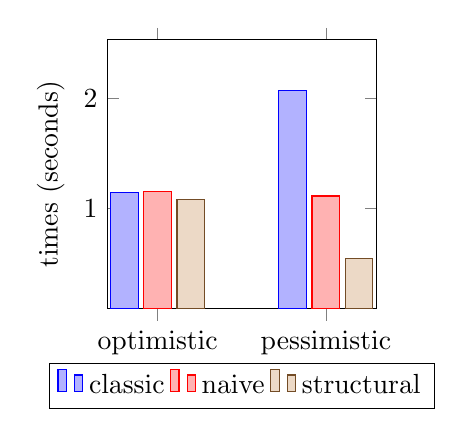
\begin{tikzpicture}
\begin{axis}[
    ybar,
    enlargelimits=0.3,
    width=5cm, height=5cm,
    legend style={at={(0.5,-0.2)},
      anchor=north,legend columns=-1},
    ylabel={times (seconds)},
    symbolic x coords={optimistic, pessimistic},
    xtick=data
    ]
\addplot coordinates {(optimistic,1.142) (pessimistic,2.073)};
\addplot coordinates {(optimistic,1.151) (pessimistic,1.110)};
\addplot coordinates {(optimistic,1.077) (pessimistic,0.542)};
\legend{classic,naive,structural}
\end{axis}
\end{tikzpicture}
  \caption{The results of revers$^o$ evaluation for a list with a length of 90}
  \label{fair:plot-reverso}
\end{figure}

\begin{figure}[h]
\centering
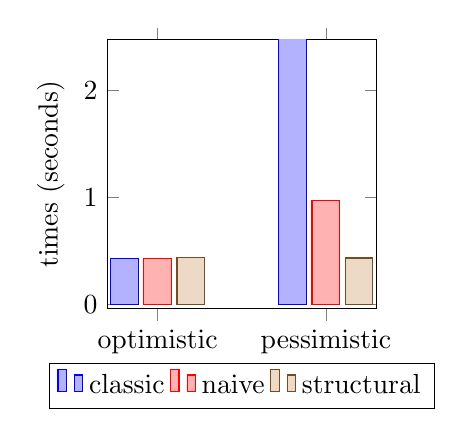
\begin{tikzpicture}
\begin{axis}[
    ybar, ymax = 2,
    enlargelimits=0.3,
    width=5cm, height=5cm,
    legend style={at={(0.5,-0.2)},
      anchor=north,legend columns=-1},
    ylabel={times (seconds)},
    symbolic x coords={optimistic, pessimistic},
    xtick=data
    ]
\addplot coordinates {(optimistic,0.430) (pessimistic,300)};
\addplot coordinates {(optimistic,0.428) (pessimistic,0.969)};
\addplot coordinates {(optimistic,0.433) (pessimistic,0.432)};
\legend{classic,naive,structural}
\end{axis}
\end{tikzpicture}
\caption{The results of sort$^o$ evaluation for a list with a length of 5}
\label{fair:plot-sorto}
\end{figure}

\begin{figure}[h]
\centering
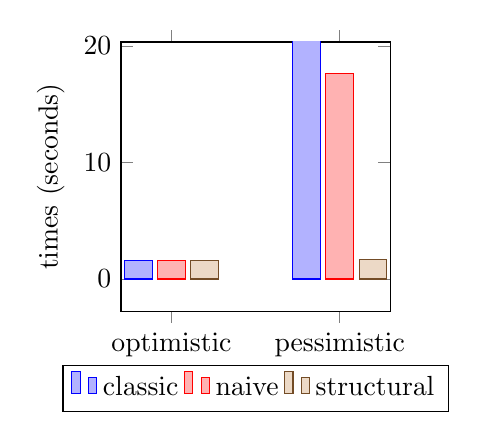
\begin{tikzpicture}
\begin{axis}[
    ybar, ymax = 16,
    enlargelimits=0.3,
    width=5cm, height=5cm,
    legend style={at={(0.5,-0.2)},
      anchor=north,legend columns=-1},
    ylabel={times (seconds)},
    symbolic x coords={optimistic, pessimistic},
    xtick=data
    ]
\addplot coordinates {(optimistic,1.574) (pessimistic,300)};
\addplot coordinates {(optimistic,1.579) (pessimistic,17.604)};
\addplot coordinates {(optimistic,1.585) (pessimistic,1.646)};
\legend{classic,naive,structural}
\end{axis}
\end{tikzpicture}
\caption{The results of ``The Tower of Hanoi'' solver}
\label{fail:plot-hanoi}
\end{figure}

\begin{figure}[h]
\centering
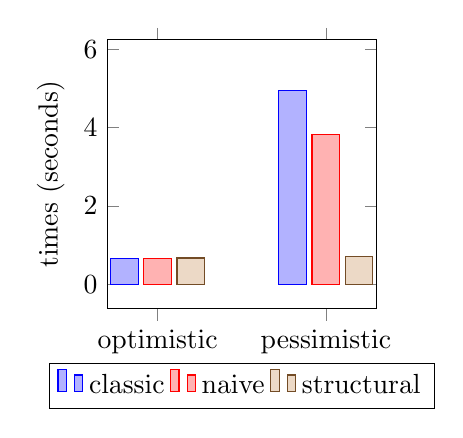
\begin{tikzpicture}
\begin{axis}[
    ybar,
    enlargelimits=0.3,
    width=5cm, height=5cm,
    legend style={at={(0.5,-0.2)},
      anchor=north,legend columns=-1},
    ylabel={times (seconds)},
    symbolic x coords={optimistic, pessimistic},
    xtick=data
    ]
\addplot coordinates {(optimistic,0.669) (pessimistic,4.956)};
\addplot coordinates {(optimistic,0.663) (pessimistic,3.820)};
\addplot coordinates {(optimistic,0.675) (pessimistic,0.712)};
\legend{classic,naive,structural}
\end{axis}
\end{tikzpicture}
\caption{The results of ``Bridge and torch problem'' solver}
\label{fair:plot-bridge}
\end{figure}

\begin{figure}[h]
  \small
  \centering
  \begin{tabular}{ c | c | c | c | c | c | c | c }
    \multirow{2}{*}{relation} & \multirow{2}{*}{size} & 
    \multicolumn{2}{c}{classic conjunction} &
    \multicolumn{2}{c}{naive fair conjunction} &
    \multicolumn{2}{c}{fair conjunction} \\
    \cline{3-8}
    & & optimistic & pessimistic & optimistic & pessimistic & optimistic & pessimistic  \\ 
    \hline
    \multirow{3}{*}{revers$^o$}
                 & 30   & 0.465 & 0.532 & 0.468 & 0.461  & 0.438 & 0.425 \\
                 & 60   & 0.579 & 0.828 & 0.577 & 0.658  & 0.545 & 0.450 \\
                 & 90   & 1.142 & 2.073 & 1.151 & 1.110  & 1.077 & 0.542 \\
    \hline
    \multirow{5}{*}{sort$^o$}
                 & 3    & 0.418 & 0.432 & 0.420 & 0.420  & 0.424 & 0.425 \\
                 & 4    & 0.424 & 3.924 & 0.424 & 0.455  & 0.429 & 0.429 \\
                 & 5    & 0.430 & >300  & 0.428 & 0.969  & 0.433 & 0.432 \\
                 & 6    & 0.434 & >300  & 0.430 & 11.577 & 0.434 & 0.437 \\
                 & 30   & 1.664 & >300  & 1.636 & >300   & 1.723 & 1.751 \\ 
    \hline
    hanoi$^o$    & -    & 1.574 & >300  & 1.579 & 17.604 & 1.585 & 1.646 \\
    \hline
    bridge$^o$   & -    & 0.669 & 4.956 & 0.663 & 3.820 & 0.675 & 0.712    

  \end{tabular}
  \caption{The results of an evaluation: running times of benchmarks in seconds}
  \label{fair:evaluation-table}
\end{figure}